% The contents of this file is 
% Copyright (c) 2015- David S. Read, All Rights Reserved

\chapter{Object Oriented Notes}

\label{ooconcepts}

\section{Instances}
%\textbf{\underline{Instances}}

\index{instance}
\index{object}
\index{keyword!new}
\index{new keyword}

You may have noticed something different about the way we use some classes, such as Random, in our code. For example see the program in section \ref{usingRandomInstance} on page \pageref{usingRandomInstance} which demonstrates the generation of random numbers. 

The program includes the following line:

\texttt{Random randomGenerator = new Random();}

What does this statement do? Also, why, when we go to use the \texttt{nextFloat} method, do we call it like this:

\texttt{randomGenerator.nextFloat()}

This brings us squarely into the realm of objects (remember Java is an object-oriented language). Usually the methods in a class are written to be called using an object, known as an instance of the class. It'll take a while to clarify how objects work. 

For now think of objects as providing a way that Java sets aside memory so that the methods can store and retrieve information they need to do their jobs. We use the keyword \texttt{new} to tell Java what class we want to create an object from. We get back an object that we can then call methods on.

Here are a couple of classes we can use to depict this relationship of class, object (instance of the class), attributes and methods

First, here is a class called \texttt{Point}. It is designed to store an \textbf{X} and \textbf{Y} coordinate:


\beforeverb
\begin{verbatim}
public class Point {
public int myX;
public int myY;

public void setXandY(int updatedX, int updatedY) {
myX = updatedX;
myY = updatedY;
}

public int getX() {
return myX;
}

public int getY() {
return myY;
}
}
\end{verbatim}
\afterverb

Looking at the \texttt{Point} class you'll see that it declares two attributes, \texttt{myX} and \texttt{myY}. They are declared inside the class and outside of a method which is what makes them attributes of the class. For each instance of the \texttt{Point} class these variable will be assigned different memory locations by the computer, allowing them to store different values for \textbf{X} and \textbf{Y} coordinates.

The method \texttt{setXAndY} takes two arguments. They are named \texttt{updatedX} and \texttt{updatedY}. Looking at the code in the method we see that the value in \texttt{updatedX} is assigned to the attribute \texttt{myX} and the value in \texttt{updatedY} is assigned to the attribute \texttt{myY}. 

The other two methods in the \texttt{Point} class, \texttt{getX} and \texttt{getY}, return the value of \texttt{myX} and \texttt{myY}, respectively.

Note that the \texttt{Point} class doesn't contain a \texttt{main} method. This class is used to store information (X and Y coordinates) and is not a complete program. Rather, it can be used by a program to store X and Y locations.

\newpage

Now let's write another class that uses instances of the \texttt{Point} class to store multiple coordinates:

\beforeverb
\begin{verbatim}
public class WorkWithPoints {
public static void main(String[] args) {
// Declare variables of type Point
Point firstPoint;
Point secondPoint;
Point whatIsThePoint;

// Create instances of the Point class
firstPoint = new Point();
secondPoint = new Point();
whatIsThePoint = new Point();

// Call the setXandY method on each Point instance
firstPoint.setXandY(1, 2);
secondPoint.setXandY(3, 4);
whatIsThePoint.setXandY(5, 6);

// Display some X and Y values from the Point instances
System.out.println(firstPoint.getY());
System.out.println(secondPoint.getX());
System.out.println(whatIsThePoint.getY());
}
}
\end{verbatim}
\afterverb

The \texttt{WorkWithPoints} class has a single method, \texttt{main}. This is the method that will run when we start our program. You can see that the method starts off by declaring three variables, \texttt{firstPoint}, \texttt{secondPoint} and \texttt{whatIsThePoint}. Each variable's type is \texttt{Point}, which is the class we just looked at, above. 

The next several lines in \texttt{WorkWithPoints} create instances of the \texttt{Point} class. The keyword \texttt{new} is used to create an instance of a class. Following the \texttt{new} keyword is the name of the class treated as a method (e.g. with parentheses after it)\footnote{This isn't quite correct but we'll learn about constructors later. What is correct is that using the \texttt{new} keyword creates an object, an instance of the named class.}

The \texttt{main} method then has statements which call the \texttt{setXAndY} method on each instance, sending different argument values in each case. Remember that \texttt{Point} instances can hold two integers representing the X and Y coordinates of a point. These are stored in the attributes names \texttt{myX} and \texttt{myY}. The first point that is set is given the coordinates (1, 2), the second is set to (3, 4) and the last one is set to the coordinates (5, 6).

The last few lines of the \texttt{WorkWithPoints main} method output a few of the X and Y values to the screen.

\textit{Let's turn our attention to how we can create three Point instances which will allow us to store and access three separate sets of coordinates.}

Remember that each object is given main memory to store its attributes. Each \texttt{Point} instance will have a \texttt{myX} and \texttt{myY} variable to store, so each \texttt{Point} object will reserve space for those. Since we create three \texttt{Point} objects, we will have space to store values for three \texttt{myX} attributes and three \texttt{myY} attributes.

We are left with one issue, when we call the \texttt{setXandY} method, how does it know \textbf{\textit{which object's attributes to set}}? Look carefully at the statements in the \texttt{main} method that call the \texttt{setXandY} method. Here they are for clarity:

\beforeverb
\begin{verbatim}
firstPoint.setXandY(1, 2);
secondPoint.setXandY(3, 4);
whatIsThePoint.setXandY(5, 6);
\end{verbatim}
\afterverb

What is placed in front of each call to the \texttt{setXandY} method? It is the name of one of the variables that is holding a \texttt{Point} instance! We tell Java which instance to run the method on by naming the instance's variable first and then naming the method second. We place a dot between the two so that Java can easily tell the variable name from the method name.

The depiction below is meant to show the contents of memory once the \texttt{main} method reaches the \texttt{System.out.println} method calls.

\beforefig
\centerline{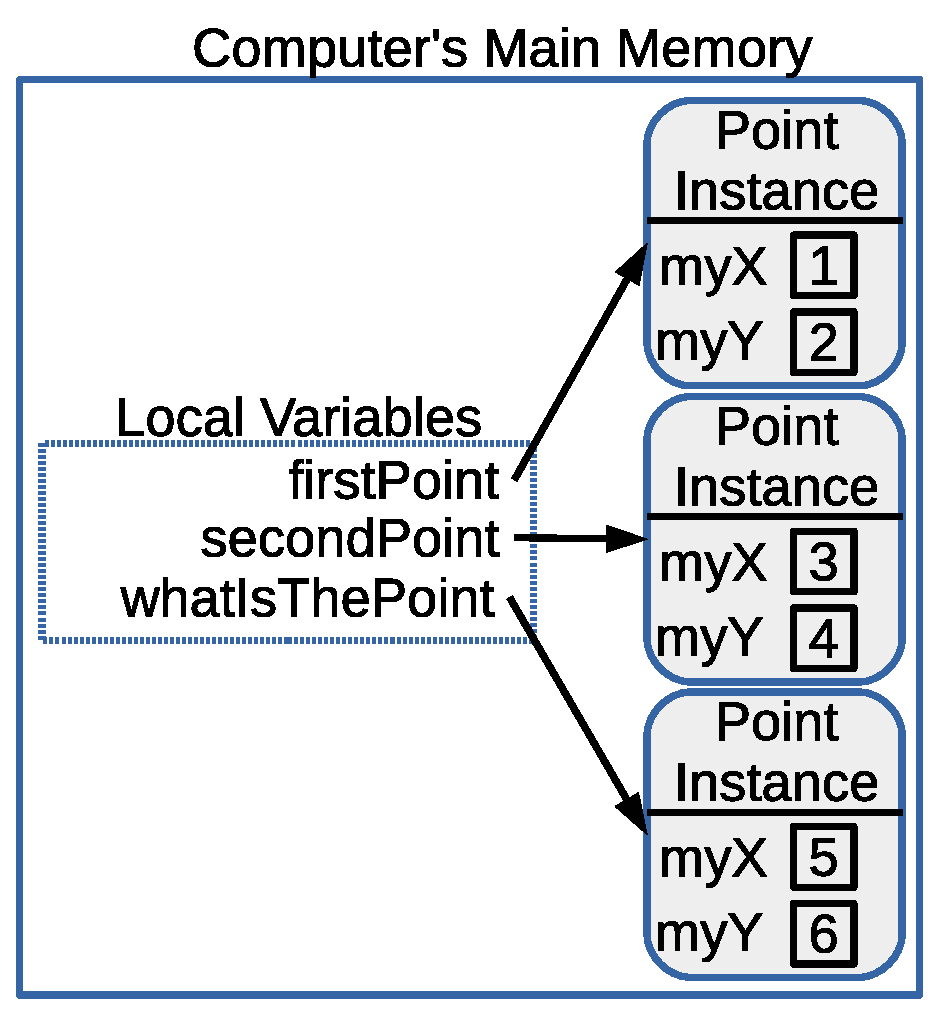
\includegraphics[height=2.25in]{figs2/ObjectsAndAttributes.eps}}
\afterfig

Given this understanding can you predict what will be printed on the screen when the \texttt{WorkWithPoints} class is run? 

As a reminder, these are the three print statements from above:

\beforeverb
\begin{verbatim}
System.out.println(firstPoint.getY());
System.out.println(secondPoint.getX());
System.out.println(whatIsThePoint.getY());
\end{verbatim}
\afterverb

Look carefully at which instance variables are being used with the \texttt{getX} and \texttt{getY} method calls in the \texttt{System.out.println} calls.

To check your understanding, here is the program's output:

\beforeverb
\begin{verbatim}
2
3
6
\end{verbatim}
\afterverb


The above example is meant as a high-level depiction of how classes, objects (instances), attributes and methods relate. Covering all the concepts related to object-oriented programming in detail will require a chapter all its own, so be patient, you'll get it.
